%\addtocounter{chapter}{-1}
\chapter{Advice for the Reader}

\section{Prerequisites}
This book is intended to be accessible to anyone with a basic understanding of
high school level mathematics.
In particular, the reader is not expected to know anything about higher maths,
computer science or programming.

Some fundamental ideas that surpass this scope shall be introduced in
\Cref{part:foundations}. If you already understand them,
you are welcome to skip this part.

\section{Deciding What to Read}
There is no need to read this book in linear order:
it covers all sorts of areas in computer science, as well as the supporting
mathematical foundations required for each of them. There are many possible
paths to progress through them, and the order in which they are presented here
is merely the one I find most comfortable. \Cref{ch:sales} gives a short
overview of what to expect in which chapter and what a given subject or area
deals with.

% TODO: Dependency Graph?

\section{Questions, Exercises and Problems}
This book, much like the original \emph{Infinite Napkin\cite{ref:napkin}} has
three levels of exercises:
\begin{itemize}
  \ii{} An inline \vocab{question} is intentionally easy. These are largely
        there to give you a chance to internalize and understand definitions.
        If you find yourself unable to answer a few of them, it probably means
        that I've explained things badly and you should complain to me.
        If you find yourself not understanding many, you've likely missed an
        important point or forgot to check out a prerequisite chapter: circle
        back there and try again.
  \ii{} An inline \vocab{exercise} has more to it than a question, usually in
        the form of additional steps, but there shouldn't be any ``difficult''
        steps.
        These might be proofs of theorems or propositions, assuming they are
        instructive and interesting enough to warrant inclusion in this book.
  \ii{} Each chapter also features several \vocab{problems} at the end.
        Some are reasonably easy to resolve still, but others are legitimately
        difficult problems for a college-level student who is taking the course
        to solve. None of them will be quite as difficult as the
        ``olympiad-level'' problems in the original \emph{Infinite
        Napkin\cite{ref:napkin}}.
        \onechili{} Harder problems will be marked with up to three chili peppers
        (\scalebox{0.7}{\chili}), like this paragraph.

        In addition to difficulty annotations, the problems are also marked by
        how important they are in the grand scheme of things.
        \begin{itemize}
          \ii{}\textbf{Normal problems},
          which may be interesting, but not essential.
          \ii{}\textbf{Daggered problems},
          which are results that one should be aware of, but that aren't
          essential to understand later parts of this book.
          \ii{}\textbf{Starred problems},
          which are results that will be used later on.
        \end{itemize}
\end{itemize}
Several hints and solutions can be found in \Cref{app:hints,app:sol}.

\section{Paper}
As with the original work\cite{ref:napkin},
\begin{moral}
  Read this book with pencil and paper.
\end{moral}
Here's why:

\begin{center}
  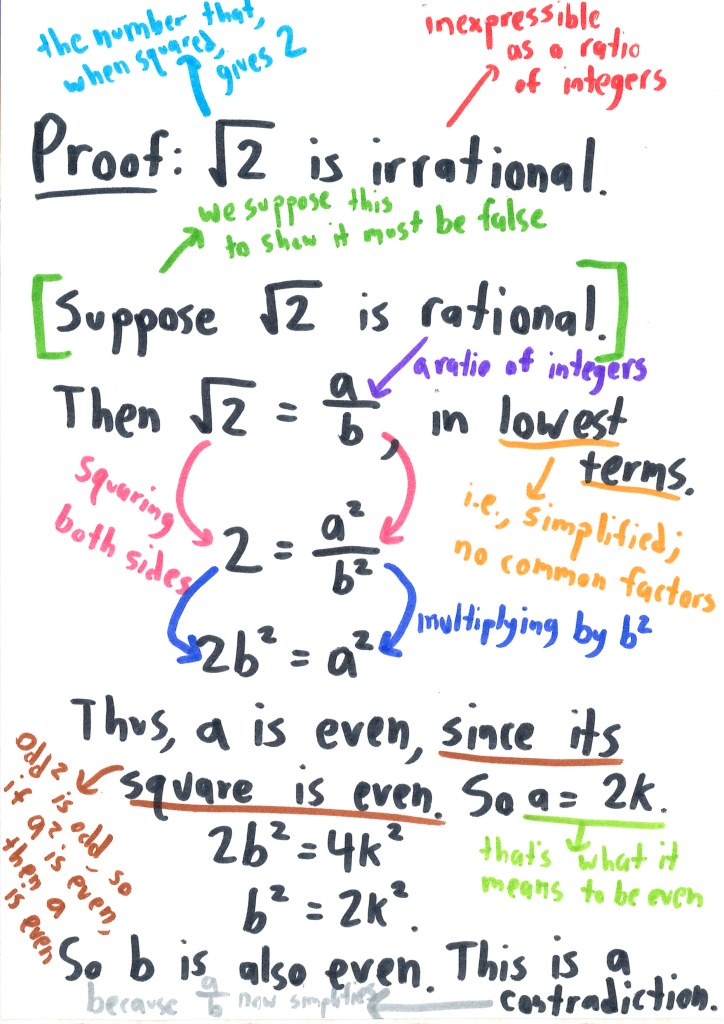
\includegraphics[width=0.5\textwidth]{media/read-with-pencil.jpg}
  \\ \scriptsize Image from~\cite{img:read_with_pencil}
\end{center}
You are not God.
You cannot keep everything in your head.\footnote{See also
	\url{https://blog.evanchen.cc/2015/03/14/writing/} and the source above.}
If you've printed out a hard copy, then write in the margins.
If you're trying to save paper,
grab a notebook or something along with the ride.
Somehow, some way, make sure you can write. Thanks.

\section{Further Reading}
The appendix \Cref{ch:refs} contains a list of resources I like,
and explanations of pedagogical choices that I made for each chapter.
I encourage you to check it out.

In particular, this is where you should go for further reading!
There are some topics that should be covered in the Napkin,
but are not, due to my own ignorance or laziness.
The references provided in this appendix should hopefully help partially
atone for my omissions.

\section{Why Are There Two Maths Sections?}
You might have noticed that this book has two separate sections on mathematics.
That's because many people, at least according to their own (often misguided)
opinion, \emph{do not like maths}. Hence, I have decided to separate into two
distinct sections those portions of mathematics I consider \emph{absolutely
  essential} and those which are required only for certain applications or
fields, or for further studies in certain areas.
